\documentclass[10pt,compress]{beamer}
\usetheme[hideothersubsections]{Berkeley}
\definecolor{aggiemaroon}{RGB}{80,0,0}
\usecolortheme[named=aggiemaroon]{structure}
\useoutertheme{shadow}
\useinnertheme{rounded}
\setbeamertemplate{navigation symbols}{}
\setbeamertemplate{mini frames}{}
\setbeamertemplate{headline}{}
\setbeamerfont{structure}{family=\rmfamily,series=\bfseries}
\usefonttheme[stillsansseriftext]{serif}

\usepackage{amsmath,amssymb,bm}
\usepackage{graphicx}
\usepackage{tikz}
\usetikzlibrary{positioning,arrows.meta,calc}
\usepackage{multicol}
\usepackage{hyperref}
\usepackage{booktabs}
\usepackage{array}
\usepackage{mathtools}

\newcommand{\R}{\mathbb{R}}
\newcommand{\E}{\mathbb{E}}
\newcommand{\prob}{\mathbb{P}}
\newcommand{\norm}[1]{\lVert #1\rVert}
\newcommand{\kpt}{\bm{x}}
\newcommand{\means}{\bm{u}}

% Compact inline gloss for symbols in an equation just shown -- NOT a
% separate slide, just a small note directly under the math.
\newcommand{\defline}[1]{{\footnotesize\textcolor{aggiemaroon}{\textit{#1}}\par}}

\title[k-means: MacQueen (1967)]{Some Methods for Classification and Analysis of Multivariate Observations}
\subtitle{A plain-language walkthrough of MacQueen's k-means paper}
\author[Thomas]{Nathaniel Thomas}
\date[September 26, 2026]{September 26, 2026}
\institute[Texas A\&M University]{Texas A\&M University}

\begin{document}

\begin{frame}
  \titlepage
\end{frame}

\begin{frame}{Overview}
\tableofcontents
\end{frame}

% ------------------------------------------------------------------
\section[Problem]{Problem and formulation}

\begin{frame}{1. What problem is MacQueen actually solving?}
The paper begins with a population in $\R^N$ and asks for a partition into $k$ groups having low \emph{within-class variance}.
\defline{$\R^N$: a data point with $N$ numbers, e.g.\ $(3,-1,7)$ if $N=3$.}

For a partition $S=\{S_1,\ldots,S_k\}$ with conditional means $u_i$, MacQueen defines
\[
W^2(S)=\sum_{i=1}^k \int_{S_i}\norm{z-u_i}^2\,dp(z).
\]
\defline{$S_i$: group $i$ (the $k$ groups cover everyone, no overlaps). $u_i$: true average of the points in $S_i$. $\int(\cdot)\,dp(z)$: ``average over all points $z$, weighted by how likely each one is.''}
\begin{itemize}\small
\item $W^2(S)$: a measure of how spread out the points are within each group.
\item Small $W^2(S)$ = tight, well-separated groups; the goal is to find a good partition \emph{without} solving this exactly.
\end{itemize}
\vfill
{\scriptsize MacQueen, pp.~281--282, Sec.~1.}
\end{frame}


\begin{frame}{2. The minimum-distance partition}
Given $\kpt=(x_1,\ldots,x_k)$ (a guess at the $k$ group centers), define the Voronoi-like cells

\[
T_i(\kpt)=\{z\in\R^N:\norm{z-x_i}<\norm{z-x_j},\ j\neq i\}.
\]
\defline{$\norm{z-x_i}$: ordinary distance from point $z$ to center $x_i$. $T_i$: all points strictly closer to $x_i$ than to any other center.}
MacQueen makes a tie-breaking rule and sets $S_1=T_1,\ S_2=T_2\setminus S_1,\ldots$ so every point lands in exactly one group.
\begin{columns}[T]
\column{0.48\textwidth}
\begin{center}
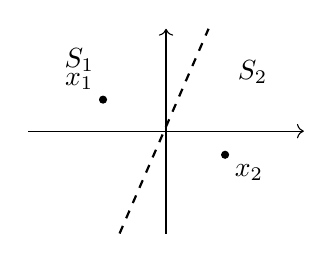
\begin{tikzpicture}[scale=0.5]
\draw[->] (-3.5,0)--(3.5,0);
\draw[->] (0,-2.6)--(0,2.6);
% Perpendicular bisector of the segment joining the two centers.
\draw[thick,dashed] (-1.18,-2.6)--(1.08,2.6);
\filldraw[black] (-1.6,0.8) circle (2.5pt) node[above left] {$x_1$};
\filldraw[black] (1.5,-0.6) circle (2.5pt) node[below right] {$x_2$};
\node at (-2.2,1.8) {$S_1$};\node at (2.2,1.5) {$S_2$};
\end{tikzpicture}
\end{center}
{\scriptsize MacQueen, pp.~282--283, Eqs.~(2.1)--(2.2).}
\column{0.48\textwidth}
\footnotesize Every point is colored by the center it's closest to; the dashed line (equidistant points) is the group boundary.
\begin{center}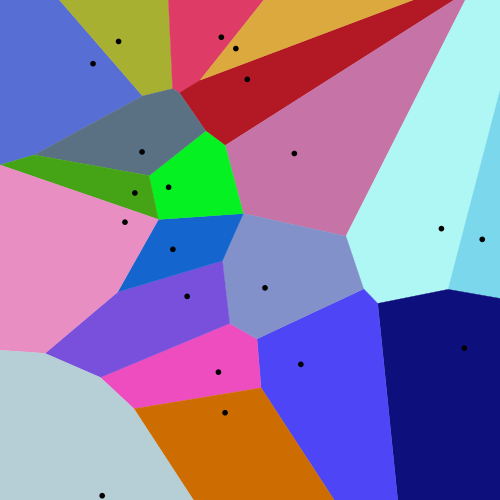
\includegraphics[width=0.45\textwidth]{voronoi.png} \par\end{center}
A Voronoi diagram taken from \url{https://en.wikipedia.org/wiki/Voronoi_diagram}
\end{columns}
\vfill
\end{frame}

\begin{frame}{3. Guessed centers vs.\ true means}
For a $k$-point $\kpt$ (a list of $k$ candidate centers), MacQueen compares
\[
W(\kpt)=\sum_{i=1}^k\int_{S_i(\kpt)}\norm{z-x_i}^2\,dp(z),
\]
\[
V(\kpt)=\sum_{i=1}^k\int_{S_i(\kpt)}\norm{z-u_i(\kpt)}^2\,dp(z).
\]
\defline{$W$: error using our \emph{guessed} centers $x_i$. $V$: error using the \emph{true} cell means $u_i(\kpt)$ instead -- always at least as good, so $V(\kpt)\le W(\kpt)$.}
Since $\int_{S_i}\norm{z-x_i}^2dp=\int_{S_i}\norm{z-u_i}^2dp+p(S_i)\norm{x_i-u_i}^2$, we get
\[
W(\kpt)=V(\kpt)+\sum_i p(S_i)\norm{x_i-u_i}^2.
\]
\defline{Reason: write $z-x_i=(z-u_i)+(u_i-x_i)$. The cross term vanishes because $u_i$ is the conditional mean on $S_i$, so $\int_{S_i}(z-u_i)\,dp(z)=0$. The remaining term is the squared bias $p(S_i)\norm{x_i-u_i}^2$.}
\defline{$p(S_i)$: fraction of the population in group $i$. This is a bias--variance split: total error = error with the perfect center + penalty for how wrong the guess is.}
\vfill
{\scriptsize MacQueen, pp.~283, 286--287, Eqs.~(2.3), (2.16).}
\end{frame}

% ------------------------------------------------------------------
\section[Online process]{The online k-means process}

\begin{frame}{4. MacQueen's sample k-means algorithm}
Let $Z_1,Z_2,\ldots$ be observations from $p$ (drawn independently, all from the same distribution). Initialize $x_i^1=Z_i,\ w_i^1=1$ for $i=1,\ldots,k$. For each new point $Z_{k+n}$:
\begin{enumerate}\small
\item Find its nearest current mean $x_i^n$ and join that group; increment weight $w_i^n$.
\item Update only that mean: $x_i^{n+1}=\dfrac{w_i^n x_i^n+Z_{k+n}}{w_i^n+1}$, $\ w_i^{n+1}=w_i^n+1$; all other means stay put.
\end{enumerate}
\defline{$w_i^n$: how many points are currently in group $i$ -- the update is just folding one new point into a running average, like updating a class average with a new grade.}
\begin{center}
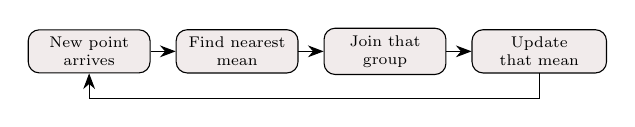
\begin{tikzpicture}[scale=0.8,transform shape,node distance=4mm, >={Stealth[length=2mm]}, every node/.style={font=\scriptsize,align=center}]
\node[draw,rounded corners,fill=aggiemaroon!8,text width=1.7cm] (a) {New point arrives};
\node[draw,rounded corners,fill=aggiemaroon!8,text width=1.7cm,right=4mm of a] (b) {Find nearest mean};
\node[draw,rounded corners,fill=aggiemaroon!8,text width=1.7cm,right=4mm of b] (c) {Join that group};
\node[draw,rounded corners,fill=aggiemaroon!8,text width=1.9cm,right=4mm of c] (d) {Update that mean};
\draw[->] (a)--(b); \draw[->] (b)--(c); \draw[->] (c)--(d);
\draw[->] (d.south) |- ++(0,-4mm) -| (a.south);
\end{tikzpicture}
\end{center}
\vfill
{\scriptsize MacQueen, p.~283, Eqs.~(2.1)--(2.2).}
\end{frame}

% ------------------------------------------------------------------
\section[Convergence]{Convergence theorem}

\begin{frame}{5. Theorem 1: what converges?}
\begin{block}{\footnotesize MacQueen's principal result}
\small The sequence $W(x^1),W(x^2),\ldots$ converges almost surely (a.s.\ = with probability 1). Its limit is a.s.\ equal to $V(x)$ for some $k$-point $x$ whose components are distinct and \emph{unbiased}: $x_i=u_i(x)$ for every $i$, where $u_i(x)$ is the true mean of cell $S_i(x)$.
\end{block}
\defline{In words: feed the algorithm more data and the error score settles to one fixed number; at that point each guessed center exactly equals the true average of its own group.}
\begin{alertblock}{\footnotesize What it does \emph{not} say}
\small It does not say the algorithm finds the globally optimal partition -- MacQueen gives examples where it converges, with positive probability, to a configuration whose $V$ is not minimal.
\end{alertblock}
\vfill
{\scriptsize MacQueen, p.~283, Theorem 1; pp.~287--288, Sec.~2.3.}
\end{frame}

\begin{frame}{6. Theorem 2: representatives become self-consistent}
With $p_i^n=p(S_i(x^n))$ (size of group $i$ at step $n$) and $u_i^n=u_i(x^n)$ (its true mean at step $n$), MacQueen shows
\[
\frac{1}{m}\sum_{n=1}^{m}\sum_{i=1}^{k}
 p_i^n\norm{x_i^n-u_i^n}\;\longrightarrow\;0 \quad\text{a.s.}
\]
\defline{Averaged over time, the size-weighted gap between guessed and true centers shrinks to zero: big groups can't stay permanently mis-centered. This is a Ces\`aro (time-averaged) statement -- individual steps can still wobble.}
\vfill
{\scriptsize MacQueen, p.~283, Theorem 2 and p.~287.}
\end{frame}

\begin{frame}{7. Why $W(x^n)$ converges: proof sketch}
Let $\mathcal F_n$ be everything observed through step $n$. The key step compares $\E[W(x^{n+1})\mid\mathcal F_n]$ (expected error at the next step, given the past) with $W(x^n)$, producing an error-reducing term plus a small summable remainder; a martingale lemma then forces convergence.
\defline{A martingale is a process whose expected next value equals its current value (a fair game). Here $W(x^n)$ can only drift down or stay flat on average -- and since it can't go below zero, it has nowhere left to go but to settle.}
\begin{block}{Conceptual picture}
\small $W$ behaves like a stochastic Lyapunov function -- an ``energy'' the process reliably drains, with only finite total upward wiggle-room.
\end{block}
\vfill
{\scriptsize MacQueen, pp.~285--287, Lemma 3 and Eqs.~(2.5)--(2.14).}
\end{frame}

\begin{frame}{8. Identifying the limit: from $W$ to $V$}
Take a subsequence $x^{n_r}\to x$ that settles down (one always exists since guesses live in a bounded region). Using $W(x)=V(x)+\sum_i p(S_i(x))\norm{x_i-u_i(x)}^2$ and the fact that Theorem 2 already forces that extra term to vanish at the limit, MacQueen concludes
\[
W_0=W(x)=V(x),\qquad x_i=u_i(x)\ \text{for every positive-mass cell.}
\]
\defline{The ``bias'' penalty from slide 3 disappears at the limit, so guessed centers exactly equal true means there: the limit is an unbiased $k$-point for the population's nearest-mean partition.}
\vfill
{\scriptsize MacQueen, pp.~287, Eqs.~(2.14)--(2.17); conclusion of Theorem 1.}
\end{frame}

% ------------------------------------------------------------------
\section[Caveats]{What convergence does and does not mean}

\begin{frame}{9. Example: convergence to a non-optimal partition}
\small Take equal probability at the four corners of a rectangle slightly longer in one direction. If the first four points arrive in a particular corner order, the two means converge to the midpoints of the long edges -- with positive probability.
\begin{columns}[T]
\column{0.46\textwidth}
\begin{center}
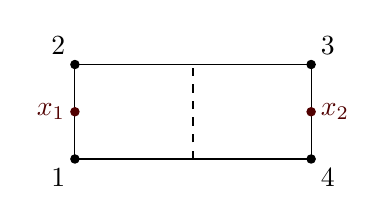
\begin{tikzpicture}[scale=0.5]
\draw (-3,-1.2) rectangle (3,1.2);
\filldraw[black] (-3,-1.2) circle (3pt) node[below left] {1};
\filldraw[black] (-3,1.2) circle (3pt) node[above left] {2};
\filldraw[black] (3,1.2) circle (3pt) node[above right] {3};
\filldraw[black] (3,-1.2) circle (3pt) node[below right] {4};
\filldraw[aggiemaroon] (-3,0) circle (3pt) node[left] {$x_1$};
\filldraw[aggiemaroon] (3,0) circle (3pt) node[right] {$x_2$};
\draw[dashed] (0,-1.2)--(0,1.2);
\end{tikzpicture}
\end{center}
\column{0.5\textwidth}
\footnotesize This split (left pair vs.\ right pair) is self-consistent but \emph{not} optimal -- the best split is top pair vs.\ bottom pair, since the rectangle is longer left-right.
\end{columns}
\small Convergence is a statement about \emph{where the process settles}, not a guarantee of global optimality.
\vfill
{\scriptsize MacQueen, p.~288.}
\end{frame}

% ------------------------------------------------------------------
\section{Applications}

\begin{frame}{10. Application 1: similarity grouping / clustering}
MacQueen's program modifies the online process with two thresholds:
\begin{description}\small
\item[$C$ (coarsening):] merge two current means if they're closer than $C$.
\item[$R$ (refinement):] if a new point is farther than $R$ from its nearest mean, make it a new mean.
\end{description}
\defline{$C$ removes near-duplicate groups; $R$ spins up a new group for genuinely new kinds of points. Together they let the number of groups adapt automatically (typically $C<R$).}
\vfill
{\scriptsize MacQueen, pp.~288--290, Sec.~3.1.}
\end{frame}

\begin{frame}{11. Application 2: nonlinear classification}
A 4-D synthetic sample: class $A$ is $(x_1{>}5,x_2{>}5)$ or $(x_1{\le}5,x_2{\le}5)$; everything else is $B$.
\defline{No single straight line separates $A$ from $B$ -- the true boundary is checkerboard-like.}
\begin{columns}[T]
\column{0.42\textwidth}
\begin{center}
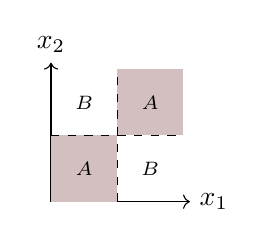
\begin{tikzpicture}[scale=0.42]
\draw[->] (0,0)--(4.2,0) node[right]{$x_1$};
\draw[->] (0,0)--(0,4.2) node[above]{$x_2$};
\fill[aggiemaroon!25] (0,0) rectangle (2,2);
\fill[aggiemaroon!25] (2,2) rectangle (4,4);
\draw[dashed] (2,0)--(2,4); \draw[dashed] (0,2)--(4,2);
\node at (1,1) {\scriptsize $A$}; \node at (3,3) {\scriptsize $A$};
\node at (3,1) {\scriptsize $B$}; \node at (1,3) {\scriptsize $B$};
\end{tikzpicture}
\end{center}
\column{0.55\textwidth}
\footnotesize k-means with $k=8$ is fit to $A$ and $B$ separately (16 means total); a new point is classified by whichever of the 16 means is nearest -- covering each class with several local ``blobs'' instead of one global rule.
\end{columns}
\begin{block}{\footnotesize Reported result}
\small 87\% correct on a new sample of 250 points.
\end{block}
\vfill
{\scriptsize MacQueen, p.~291, Sec.~3.2.}
\end{frame}

\begin{frame}{12. Application 3: approximating a distribution}
Cluster the data, fit a normal (bell-curve) distribution within each group, and mix them with weights proportional to group size.
\defline{This builds the whole population out of small bell-curve ``bumps,'' one per cluster -- usable to predict a missing coordinate or decide which population a point came from.}
In a nonlinear synthetic example (fifth coordinate $=10$ for $A$, $0$ for $B$; $k=16$):
\begin{block}{\footnotesize Reported results}
\small Standard error of estimate: 2.8. Thresholding predictions at 5 classified 96\% correctly; mean predictions were 10.3 for $A$, 1.3 for $B$.
\end{block}
\vfill
{\scriptsize MacQueen, pp.~291--292, Sec.~3.3.}
\end{frame}

\begin{frame}{13. Application 4: a scrambling test for independence}
\small Cluster the real data and record its within-class variance; then independently shuffle the values \emph{within each dimension} (keeps every marginal distribution, destroys relationships between variables) and recluster.
\defline{If shuffled data gives much higher within-class variance than the real data, that's evidence the variables really were related.}
An illustrative example (points on a square annulus, zero linear correlation but strong dependence) saw variance increase by a factor of 1.6 after scrambling, with $k=12$.
\vfill
{\scriptsize MacQueen, pp.~292--293, Sec.~3.4.}
\end{frame}

\begin{frame}{14. Application: the Forgy--Jennrich two-step method}
Starting from any partition, repeat: (1) compute each group's mean; (2) reassign every point to its nearest mean.
\defline{Each full pass can only improve (or hold) the score, and a finite dataset has only finitely many possible splits, so the loop must eventually stop.}
\begin{alertblock}{\footnotesize Relationship to modern k-means}
\small This is essentially the batch alternating-assignment/mean-update mechanism later known as Lloyd-style k-means; MacQueen treats it as a separate improvement step.
\end{alertblock}
\vfill
{\scriptsize MacQueen, p.~294, Sec.~3.6.}
\end{frame}

% ------------------------------------------------------------------
\section[Metric spaces]{Beyond Euclidean means}

\begin{frame}{15. General metric spaces: centroids replace means}
Let $(M,p)$ be a compact metric space (bounded, with a notion of distance $p$, but maybe no way to add points together). For order $r>0$, a \emph{centroid} minimizes $\int_M p(x,z)^r\,dp(z)$.
\defline{A centroid generalizes ``average'' to spaces where you can measure distance but can't literally add points (e.g.\ binary strings).}
On the real line: $r=2$ gives the ordinary mean, $r=1$ the median, $r\to\infty$ minimum-radius covering centers, $r\to0$ a mode-like point. The generalized algorithm is unchanged: swap ``mean'' for ``centroid'' everywhere, and MacQueen proves a first special case ($k=1,r=1$) of the full convergence theorem.
\vfill
{\scriptsize MacQueen, pp.~295--296, Sec.~4.}
\end{frame}

% ------------------------------------------------------------------
\section{Assessment}

\begin{frame}{16. What the paper establishes -- and leaves open}
\footnotesize
\begin{columns}[T]
\column{0.49\textwidth}
\textbf{Established}
\begin{itemize}
\item A sequential k-means procedure.
\item An unbiased fixed-point concept.
\item A.s.\ convergence of $W(x^n)$.
\item A.s.\ asymptotic self-consistency (averaged).
\item Several data-analysis procedures.
\item Extension to compact metric spaces.
\end{itemize}
\column{0.49\textwidth}
\textbf{Not established}
\begin{itemize}
\item Global optimality of the limit.
\item Uniqueness of the limiting means.
\item A convergence-rate result.
\item A universal guarantee for all distributions/metrics.
\item Proof of the full metric-space Theorem 1.
\end{itemize}
\end{columns}
\vfill
{\scriptsize Source: MacQueen, Secs.~2--4, especially pp.~287--296.}
\end{frame}

\begin{frame}{17. The conceptual arc of the paper}
\begin{center}
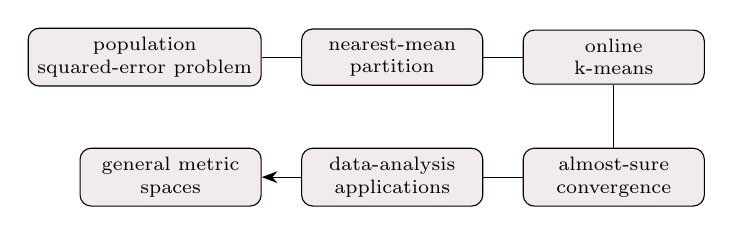
\begin{tikzpicture}[node distance=0.5cm,>={Stealth[length=2mm]},every node/.style={font=\scriptsize}]
\node[draw,rounded corners,align=center,minimum width=2.3cm,fill=aggiemaroon!8] (p) {population\\squared-error problem};
\node[draw,rounded corners,align=center,minimum width=2.3cm,fill=aggiemaroon!8,right=0.5cm of p] (v) {nearest-mean\\partition};
\node[draw,rounded corners,align=center,minimum width=2.3cm,fill=aggiemaroon!8,right=0.5cm of v] (o) {online\\k-means};
\node[draw,rounded corners,align=center,minimum width=2.3cm,fill=aggiemaroon!8,below=0.8cm of o] (t) {almost-sure\\convergence};
\node[draw,rounded corners,align=center,minimum width=2.3cm,fill=aggiemaroon!8,left=0.5cm of t] (a) {data-analysis\\applications};
\node[draw,rounded corners,align=center,minimum width=2.3cm,fill=aggiemaroon!8,left=0.5cm of a] (m) {general metric\\spaces};
\draw[->] (p)--(v)--(o)--(t)--(a)--(m);
\end{tikzpicture}
\end{center}
\defline{Read left-to-right, then right-to-left on the bottom row: define the ideal split, build an online algorithm for it, prove it settles, use it, then port the idea to more exotic spaces.}
\begin{block}{\footnotesize The central insight}
\small Each incoming point nudges its cell's center toward the true local mean. The theory shows this settles almost surely -- but not necessarily at the global optimum.
\end{block}
\vfill
{\scriptsize Synthesis of MacQueen, Secs.~1--4.}
\end{frame}

\begin{frame}{References}
\footnotesize
\begin{thebibliography}{99}
\bibitem[MacQueen, 1967]{macqueen}
J. MacQueen (1967).
\newblock Some Methods for Classification and Analysis of Multivariate Observations.
\newblock In \emph{Proceedings of the Fifth Berkeley Symposium on Mathematical Statistics and Probability}, Vol.~1, pp.~281--297.
\newblock University of California Press.

\bibitem[Forgy, 1965]{forgy}
E. Forgy (1965).
\newblock Cluster analysis of multivariate data: efficiency vs.\ interpretability of classifications.
\newblock \emph{Biometrics}, 21, p.~768 (abstract).

\bibitem[Ward, 1963]{ward}
J. Ward (1963).
\newblock Hierarchical grouping to optimize an objective function.
\newblock \emph{Journal of the American Statistical Association}, 58, 236--244.

\bibitem[Fisher, 1958]{fisher}
W. D. Fisher (1958).
\newblock On grouping for maximum homogeneity.
\newblock \emph{Journal of the American Statistical Association}, 53, 789--798.
\end{thebibliography}
\end{frame}

\begin{frame}{Take-home points}
\small
\begin{enumerate}
\item MacQueen's paper is about an \textbf{online stochastic algorithm}, not just the modern batch k-means.
\item The population objective is \textbf{within-class squared error}; conditional means are optimal for fixed cells.
\item The process converges \textbf{almost surely in objective value} under stated assumptions.
\item The limit is \textbf{unbiased/self-consistent}, but can be \textbf{non-optimal globally}.
\item The paper anticipates nonlinear classification, mixture approximation, regression, and independence testing.
\item The final section abstracts means to \textbf{centroids in general metric spaces}.
\end{enumerate}
\end{frame}

\begin{frame}{}
\centering\Huge\emph{Thank You!}
\end{frame}

\end{document}